\section{Introduction}
\label{sec:intro}
The main goal of this work is to analyze an RC circuit and study its various responses to a voltage source that changes over time. First, we studied the behavior of the circuit when the voltage imposed on the capacitor was constant and non zero (Section ~\ref{ssec:tl}), then we studied the natural response of the capacitor (voltage source imposing voltage equal to 0) in (Section ~\ref{ssec:n}), the forced response (voltage source imposing sinusoidal voltage) in (Section ~\ref{ssec:fs}), over time. We also studied the circuit for different frequencies of the sinusoidal signal, plotting the voltages at the capacitor and the nodes of its terminals as functions of frequency Section ~\ref{ssec:freq}.\\

Our circuit (Figure ~\ref{fig:circuit}) consists of 7 resistors, 2 voltage sources - 1 independent, and 1 current controlled dependent one, 1 independent current source and 1 capacitor.\\
The voltage provided by the independent source follows the equation:
\begin{equation}\label{eqn:vss}
\begin{split}
{v_s (t)} = \left\{\begin{array}{ll} \ V_s ,  \quad \ \  if \ \  \ t \leq 0 \\ 
 \ sin(2 \pi f t) , \quad \ \  if \ \ \ t \textgreater 0 \end{array} \right.
  \end{split}
\end{equation}
\begin{figure}[H] \centering
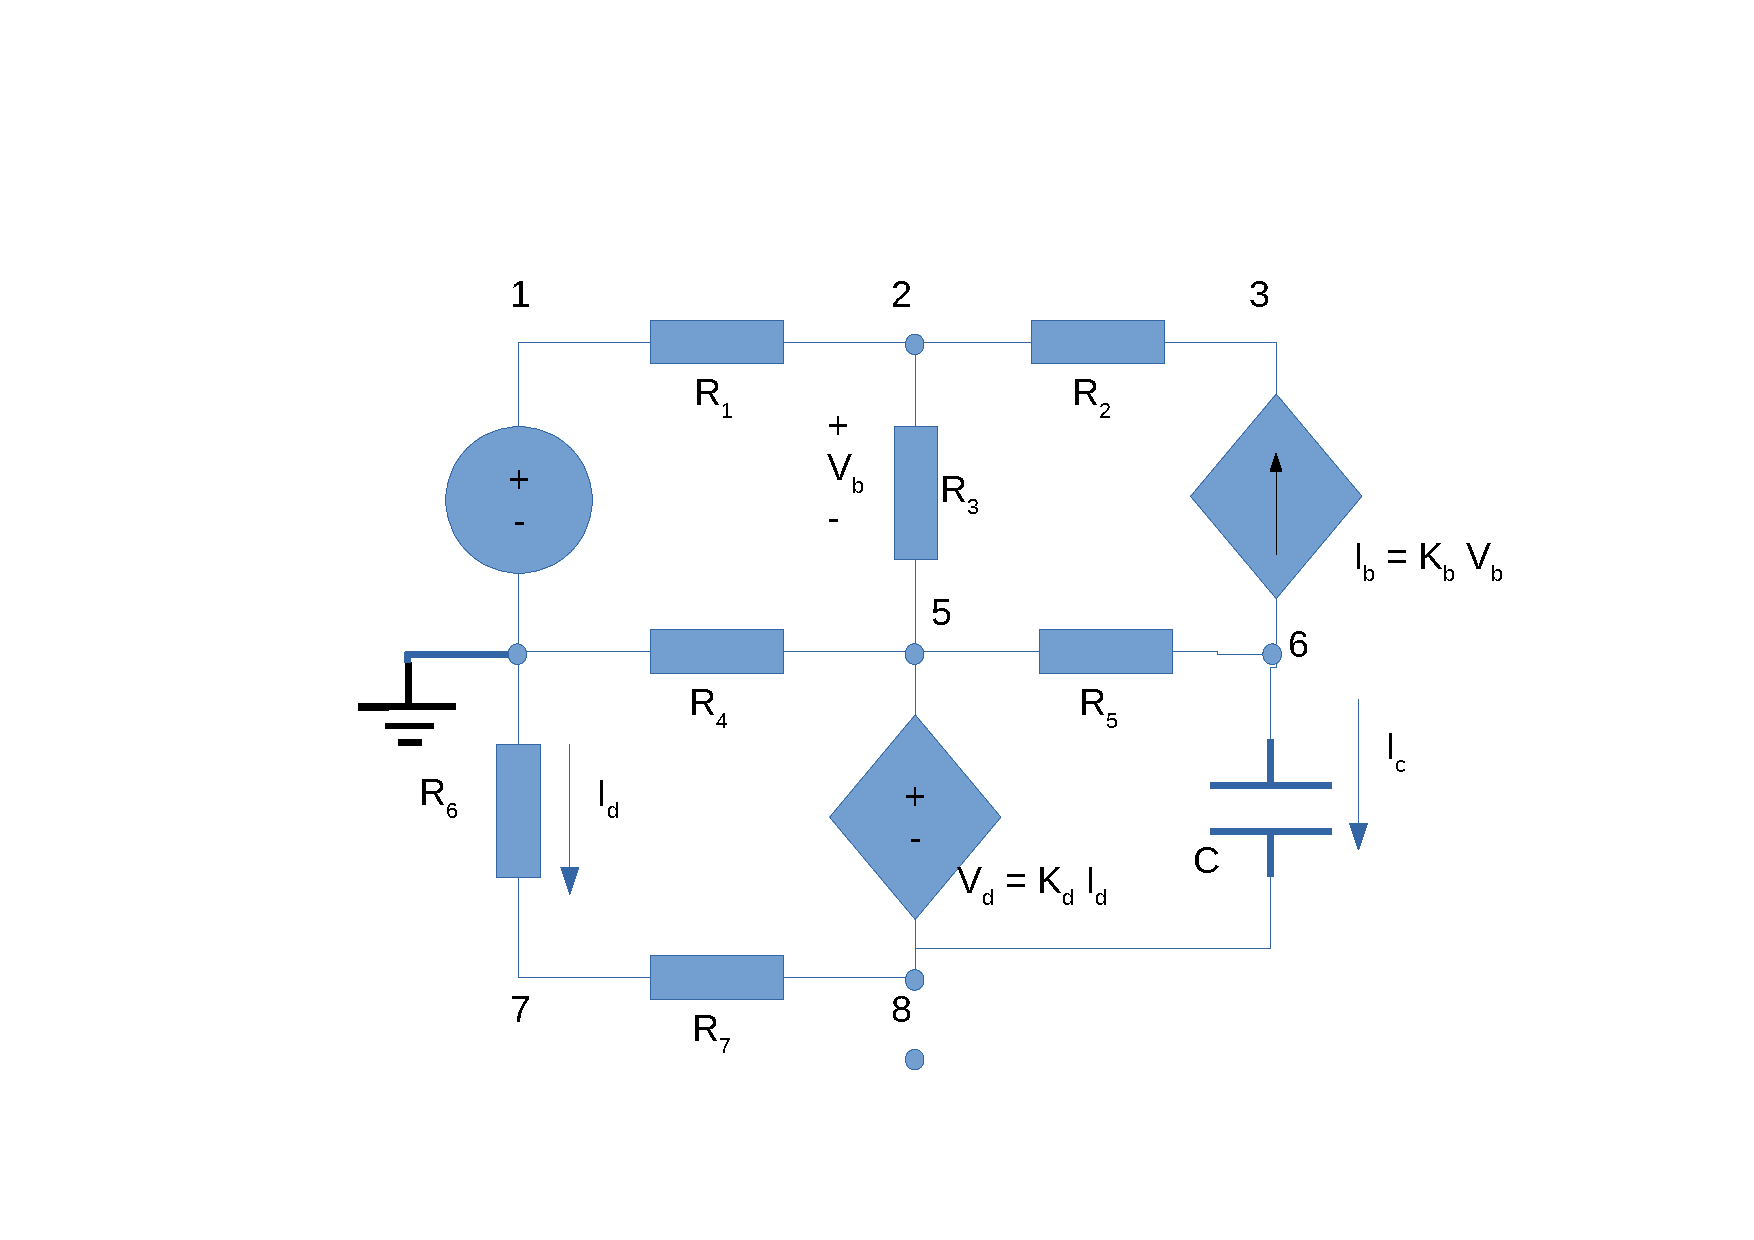
\includegraphics[width=0.8\linewidth]{circuito.pdf}
\caption{Circuit}
\label{fig:circuit}
\end{figure} 
We wrote a system of equations for each theoretical analysis, from Kirchhoff and Ohm's Laws. To get the solutions and plots for these analysis, we used \textit{octave}, which solved our systems of equations efficiently and gave us all currents and voltages for all branches. We then used \textit{ngspice} to get a simulation of this circuit, expecting to obtain the same results. We compared the results from different methods in the conclusion (Section ~\ref{sec:conclusion}).

